
%(BEGIN_QUESTION)
% Copyright 2006, Tony R. Kuphaldt, released under the Creative Commons Attribution License (v 1.0)
% This means you may do almost anything with this work of mine, so long as you give me proper credit

Make your own valve sizing problem with a given flow rate, specific gravity of liquid, upstream and downstream pressures, and an actual control valve specified from a manufacturer's product manual (e.g. Fisher ``E'' body globe valve product bulletin, or similar).  Base the given variables of your problem on the following diagram, assuming turbulent liquid flow (no choked flow conditions or any other weirdness that might necessitate a non-standard flow equation):

$$\includegraphics[width=15.5cm]{i00065x01.eps}$$

\begin{itemize}
\item{} {\bf Given conditions}
\vskip 5pt 
\item{} Flow rate $Q$ =
\vskip 5pt 
\item{} Specific gravity of liquid $G_f$ = 
\vskip 5pt 
\item{} Upstream pressure $P_1$ at specified flow rate =
\vskip 5pt 
\item{} Downstream pressure $P_2$ at specified flow rate = 
\end{itemize}

\vskip 10pt

\begin{itemize}
\item{} {\bf Proper valve for the application}
\vskip 5pt 
\item{} $C_v$ rating of valve =
\vskip 5pt 
\item{} Valve and trim suitable for the task (Manufacturer, series, part number, etc.):
\end{itemize}

\vfil

{\bf You must attach documentation from a valve manufacturer showing the suitable control valve size and type}.  Circle or highlight the relevant data on this documentation so it is clear which valve applies to your sizing problem.

\underbar{file i00065}
\eject
%(END_QUESTION)





%(BEGIN_ANSWER)

Normally I do not give hints on graded questions, but here I'll make an exception.  It might be easier to set up your problem if you {\it first} research a valve $C_v$ rating, {\it then} construct a scenario that fits the $C_v$ you were able to find.  The point of this question is to see whether or not you have mastered the basic principles of valve sizing.  It is all too easy to make up a liquid flow problem that is difficult to find a valve for, which is why I'm hinting that you ``work backwards'' from a known valve $C_v$ to the ``given'' conditions.  It may save you a lot of time, and you will still be able to prove your mastery of valve sizing calculations!

%(END_ANSWER)





%(BEGIN_NOTES)


%INDEX% Final Control Elements, valve: sizing problem

%(END_NOTES)


